\chapter{Inflation}
\label{les:9}

\begin{chapquote}{Die Königin der Herzen}
\enquote{Nun, hier muß man nämlich so schnell rennen, wie man kann, um auf der
Stelle zu bleiben. Wenn man irgendwo anders hin will, muß man mindestens doppelt
so schnell rennen.}
\end{chapquote}

Der Versuch die monetäre Inflation zu verstehen, und wie ein nicht-inflationäres
System wie Bitcoin die Dinge verändern könnte, war der Startschuss für meine
Reise in die Wirtschaft. Ich wusste, dass die Inflation die Rate war mit der
neues Geld geschaffen wurde, aber ich wusste nicht viel mehr darüber.

Während einige Ökonomen argumentieren, dass Inflation eine gute Sache ist,
argumentieren andere, dass \enquote{hartes} Geld, das nicht einfach vermehrt
werden kann — wie wir es in den Tagen des Goldstandards hatten --- für eine
gesunde Wirtschaft unerlässlich ist. Bitcoin, mit einem endlichen Vorrat von
insgesamt 21 Millionen BTC stimmt mit dem letztgenannten Lager überein.

Normalerweise sind die Auswirkungen der Inflation nicht sofort erkennbar.
Abhängig von der Inflationsrate (und anderen Faktoren) kann die Zeitdauer
zwischen Ursache und Wirkung mehrere Jahre betragen. Aber nicht nur das, die
Inflation hat sogar auf manche Gruppen von Menschen stärkeren Einfluss als auf
andere. Henry Hazlitt betont in \textit{Economics in One Lesson}: \enquote{Die
Kunst der Ökonomie besteht darin, nicht nur die unmittelbaren, sondern die
längeren Auswirkungen eines jeden Handelns oder einer Maßnahme zu betrachten;
sie besteht darin, die Folgen dieser Politik nicht nur für eine Gruppe, sondern
für alle Gruppen nachzuvollziehen.}

Einer meiner persönlichen AHA-Momente war die Erkenntnis, dass die Ausgabe neuer
Währung --- also das Drucken von mehr Geld --- eine \textit{ganz} andere
wirtschaftliche Aktivität ist, als alle anderen wirtschaftlichen Aktivitäten.
Während reale Güter und reale Dienstleistungen einen realen Wert für reale
Menschen erzeugen, tut das Drucken von Geld effektiv genau das Gegenteil: Es
mindert den Wertbestand von jedem, der die inflationierende Währung besitzt.

\begin{quotation}\begin{samepage}
\enquote{Bloße Inflation --- also die bloße Ausgabe von mehr Geld mit der Folge
höherer Löhne und Preise --- kann wie die Schaffung von mehr Nachfrage aussehen.
Aber in Bezug auf die tatsächliche Produktion und den Austausch von realen
Dingen ist es das nicht.}
\begin{flushright} -- Henry Hazlitt\footnote{Henry Hazlitt, \textit{Economics in
One Lesson} \cite{hazlitt}}
\end{flushright}\end{samepage}\end{quotation}

Die zerstörerische Kraft der Inflation wird deutlich, sobald aus ein wenig
Inflation eine \textit{ganze Menge} Inflation wird. Wenn Geld
hyperinflationiert~\cite{wiki:hyperinflation} werden die Dinge sehr schnell sehr
grässlich.\footnote{\url{https://en.wikipedia.org/wiki/Hyperinflation}} Da die
aufgeblähte Währung zusammenbricht kann sie im Laufe der Zeit keinen Wert mehr
speichern und die Menschen werden versuchen anstatt der Währung alle
möglichen Waren in die Hände zu bekommen.

\paragraph{}
Eine weitere Folge der Hyperinflation ist, dass all das Geld welches die
Menschen im Laufe ihres Lebens gespart haben verschwindet. Das Papiergeld in den
Brieftaschen wird natürlich immer noch da sein. Aber es wird genau das sein:
wertloses Papier.

\begin{figure}
  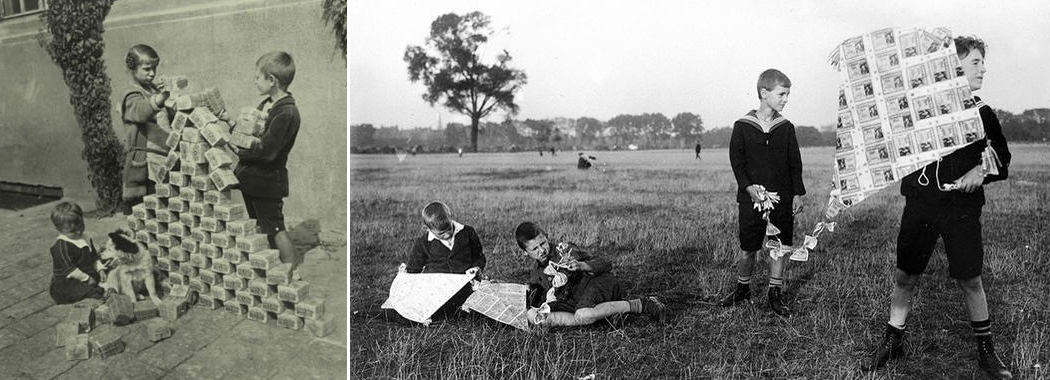
\includegraphics{assets/images/children-playing-with-money.png}
  \caption{Hyperinflation in der Weimarer Republik (1921-1923)}
  \label{fig:children-playing-with-money}
\end{figure}

\paragraph{}
Das Geld verliert auch bei einer \textit{milden} Inflation seinen Wert. Es
geschieht nur langsam genug, so dass die meisten Menschen die Abnahme der
Kaufkraft nicht bemerken. Sobald die Druckmaschinen einmal laufen ist es
schwierig die Inflation einer Währung aufzuhalten, und was soeben noch eine
milde Inflation war, kann sich per Knopfdruck in eine starke Inflation
verwandeln. Wie Friedrich Hayek in einem seiner Essays betonte, führt eine milde
Inflation in der Regel zu einer völligen Inflation.

\begin{quotation}\begin{samepage}
\enquote{Eine \enquote{milde} kontinuierliche Inflation kann nicht helfen — sie
kann nur zu einer völligen Inflation führen.}
\begin{flushright} -- Friedrich Hayek\footnote{Friedrich Hayek, \textit{1980s
Unemployment and the Unions} \cite{hayek-inflation}}
\end{flushright}\end{samepage}\end{quotation}

Die Inflation ist besonders tückisch, da sie diejenigen begünstigt die näher an
den Druckmaschinen sitzen. Es braucht Zeit bis das neu geschaffene Geld
zirkuliert und die Preise angepasst werden. Wenn du es also schaffst mehr Geld
in die Hände zu bekommen, noch bevor das aller anderen an Wert verliert, bist du
der Inflationskurve ein Stück voraus. Aus diesem Grund kann die Inflation auch
als versteckte Steuer angesehen werden, denn am Ende profitieren die Regierungen
davon während alle anderen den Preis dafür bezahlen.

\begin{quotation}\begin{samepage}
\enquote{Ich denke nicht, dass es eine Übertreibung ist zu sagen, dass die
Geschichte weitgehend eine Geschichte der Inflation ist und normalerweise die
Inflation von Regierungen für den Profit dieser Regierungen entwickelt wurde.}
\begin{flushright} -- Friedrich Hayek\footnote{Friedrich Hayek, \textit{Good
Money} (Gutes Geld) \cite{hayek-good-money}}
\end{flushright}\end{samepage}\end{quotation}

Bisher wurden alle staatlich kontrollierten Währungen ersetzt oder sind
vollständig zusammengebrochen. Egal wie gering die Inflationsrate ist,
\enquote{stetiges} Wachstum ist nur ein anderer Name für exponentielles
Wachstum. In der Natur, wie auch in der Ökonomie, werden alle Systeme die stetig
wachsen irgendwann abflachen oder einen katastrophalen Zusammenbruch
erleiden.

\paragraph{}
\enquote{Das kann in meinem Land nicht passieren} denkst du wahrscheinlich. Du
würdest das nicht denken, wenn du aus Venezuela kommst, das derzeit unter
Hyperinflation leidet. Mit einer Inflationsrate von über 1 Million Prozent ist
Geld grundsätzlich wertlos. \cite{wiki:venezuela}

\paragraph{}
Es mag sein, dass es noch nicht in den nächsten Jahren oder in deiner aktuell
benutzten Währung passiert, aber ein Blick auf die Liste der historischen
Währungen\footnote{Siehe \textit{List of historical currencies} (Liste
historischer Währungen)~\cite{wiki:historical-currencies}} zeigt,
dass dies unweigerlich über einen längeren Zeitraum geschehen wird. Ich habe
viele der aufgeführten Währungen selbst verwendet: den österreichischen
Schilling, die deutsche Mark, die italienische Lira, den französischen Franc,
das irische Pfund, den kroatischen Dinar, etc. Meine Oma benutzte sogar die
österreichisch-ungarische Krone. Im Laufe der Zeit werden die derzeit
verwendeten Währungen\footnote{Siehe \textit{List of currencies} (Liste von
Währungen)~\cite{wiki:list-of-currencies}} langsam aber sicher auf
ihre jeweiligen Friedhöfe wandern. Sie werden Hyperinflationen erleben oder
ersetzt werden. Sie werden bald historische Währungen sein. Wir werden sie
überflüssig machen.

\begin{quotation}\begin{samepage}
\enquote{Die Geschichte hat gezeigt, dass Regierungen unweigerlich der
Versuchung erliegen werden die Geldmenge zu erhöhen.}
\begin{flushright} -- Saifedean Ammous\footnote{Saifedean Ammous, \textit{Der
Bitcoin Standard} \cite{bitcoin-standard}}
\end{flushright}\end{samepage}\end{quotation}

Warum ist Bitcoin anders? Im Gegensatz zu den von der Regierung vorgeschriebenen
Währungen neigen monetäre Güter, die nicht von der Regierung sondern von den
Gesetzen der Physik\footnote{Gigi, \textit{Bitcoin's Energy Consumption - A
shift in perspective} \cite{gigi:energy}} reguliert werden, dazu zu überleben
und sogar ihren jeweiligen Wert im Laufe der Zeit zu halten. Das beste Beispiel
dafür ist Gold, das seinen Wert über Hunderte und sogar Tausende von Jahren
behält.\footnote{Ein gutes Beispiel für die Stabilität von Gold ist die
sogenannte \enquote{\textit{Gold-to-Decent-Suit Ratio}}, welche zeigt, dass man
seit jeher in etwa eine Unze Gold ausgeben muss, wenn man einen schönen Anzug
erwerben will.~\cite{web:gold-to-decent-suite-ratio}} Es ist vielleicht nicht
ganz \enquote{stabil} --- absolute Wertstabilität ist sowieso ein fragwürdiges
Konzept --- aber der Wert den es besitzt, wird in der Zukunft mindestens in
einer ähnlichen Größenordnung liegen.

Wenn ein monetäres Gut oder eine Währung den Wert über Zeit und Raum gut hält,
gilt sie als \textit{hart}. Wenn sie den Wert nicht halten kann weil sie
inflationiert oder anderweitig Wert verliert, gilt sie als \textit{weiche}
Währung. Das Konzept der Härte ist für das Verständnis von Bitcoin unerlässlich
und verdient eine gründlichere Untersuchung. Wir werden in der letzten
Wirtschaftslektion darauf zurückkommen: Solides Geld.

\paragraph{}
Da immer mehr Länder unter Hyperinflation leiden, werden mehr Menschen mit der
Realität und den Unterscheidungen von hartem und weichem Geld konfrontiert sein.
Wenn wir Glück haben, werden vielleicht sogar einige Zentralbanker gezwungen sein
ihre Geldpolitik neu zu überdenken. Was auch immer passieren mag, die
Erkenntnisse die ich dank Bitcoin gewonnen habe werden sich wahrscheinlich als
wertvoll erweisen, unabhängig vom Resultat dieser wirtschaftlichen Experimente.

\paragraph{Bitcoin lehrte mich über die versteckte Steuer der Inflation und die
Katastrophe der Hyperinflation.}

% ---
%
% #### Down the Rabbit Hole
%
% - [Economics in One Lesson][Henry Hazlitt] by Henry Hazlitt
% - [1980's Unemployment and the Unions][unions] by Friedrich Hayek
% - [Good Money, Part II][good-money]: Volume Six of the Collected Works of F.A. Hayek
% - [The Bitcoin Standard] by Saifedean Ammous
% - [Hyperinflation][hyperinflates], [economic crisis in Venezuela][wiki-venezuela], [list of historical currencies], [list of currencies][currently in use] on Wikipedia
%
% [unions]: https://books.google.com/books/about/1980s_unemployment_and_the_unions.html?id=xM9CAQAAIAAJ
% [good-money]: https://books.google.com/books?id=l_A1vVIaYBYC
%
% [Henry Hazlitt]: https://mises.org/library/economics-one-lesson
% [hyperinflates]: https://en.wikipedia.org/wiki/Hyperinflation
% [inflation cannot help]: https://books.google.com/books?id=zZu3AAAAIAAJ&dq=%22only+while+it+accelerates%22&focus=searchwithinvolume&q=%22steady+inflation+cannot+help%22
% [history of inflation]: https://books.google.com/books?id=l_A1vVIaYBYC&pg=PA142&dq=%22history+is+largely+a+history+of+inflation%22&hl=en&sa=X&ved=0ahUKEwi90NDLrdnfAhUprVkKHUx1CmIQ6AEIKjAA#v=onepage&q=%22history%20is%20largely%20a%20history%20of%20inflation%22&f=false
% [wiki-venezuela]: https://en.wikipedia.org/wiki/Crisis_in_Venezuela#Economic_crisis
% [by the laws of physics]: https://link.medium.com/9fzq2L0J3S
% [\textit{Gold-to-Decent-Suit Ratio}]: https://www.businesswire.com/news/home/20110819005774/en/History-Shows-Price-Ounce-Gold-Equals-Price
% [The Bitcoin Standard]: https://thesaifhouse.wordpress.com/book/
%
% <!-- Wikipedia -->
% [alice]: https://en.wikipedia.org/wiki/Alice%27s_Adventures_in_Wonderland
% [carroll]: https://en.wikipedia.org/wiki/Lewis_Carroll
